\documentclass[a4paper]{article}
\usepackage{amsfonts}
\usepackage{amsmath}
\usepackage{amssymb}
\usepackage{graphicx}     

\begin{document}
  
\noindent \large Auteur: Rubin Cuypers \\
\noindent \large Studierichting: Informatica\\
\noindent \large Oefeningenreeks 5F nr. 2.5\\

\medskip

\normalsize
$r_1=1$ en $ r_2^2=\cos 2 \theta$\\

opp. $r_1$:\\

$\dfrac{1}{2} \displaystyle \int_0^\pi 1 d \theta= \pi$\\

opp. $r_2$:\\

$\cos 2 \theta$ bestaat tussen $ -\dfrac{\pi}{4}$ en$ \dfrac{\pi}{4}$ en gespiegeld tussen $-\dfrac{3\pi}{4} $ en $ \dfrac{3\pi}{4}$\\

Dit kan men vereenvoudigen tot:

$ \displaystyle \int_{-\dfrac{\pi}{4}}^{\dfrac{\pi}{4}} \cos 2 \theta d\theta$\\

$= \left[\dfrac{\sin 2\theta}{2} \right]_{-\dfrac{\pi}{4}}^{\dfrac{\pi}{4}} $\\

$=1$\\

$\Rightarrow$ opp. $(r_1-r_2)= \pi-1$\\

\begin{figure}[h]
    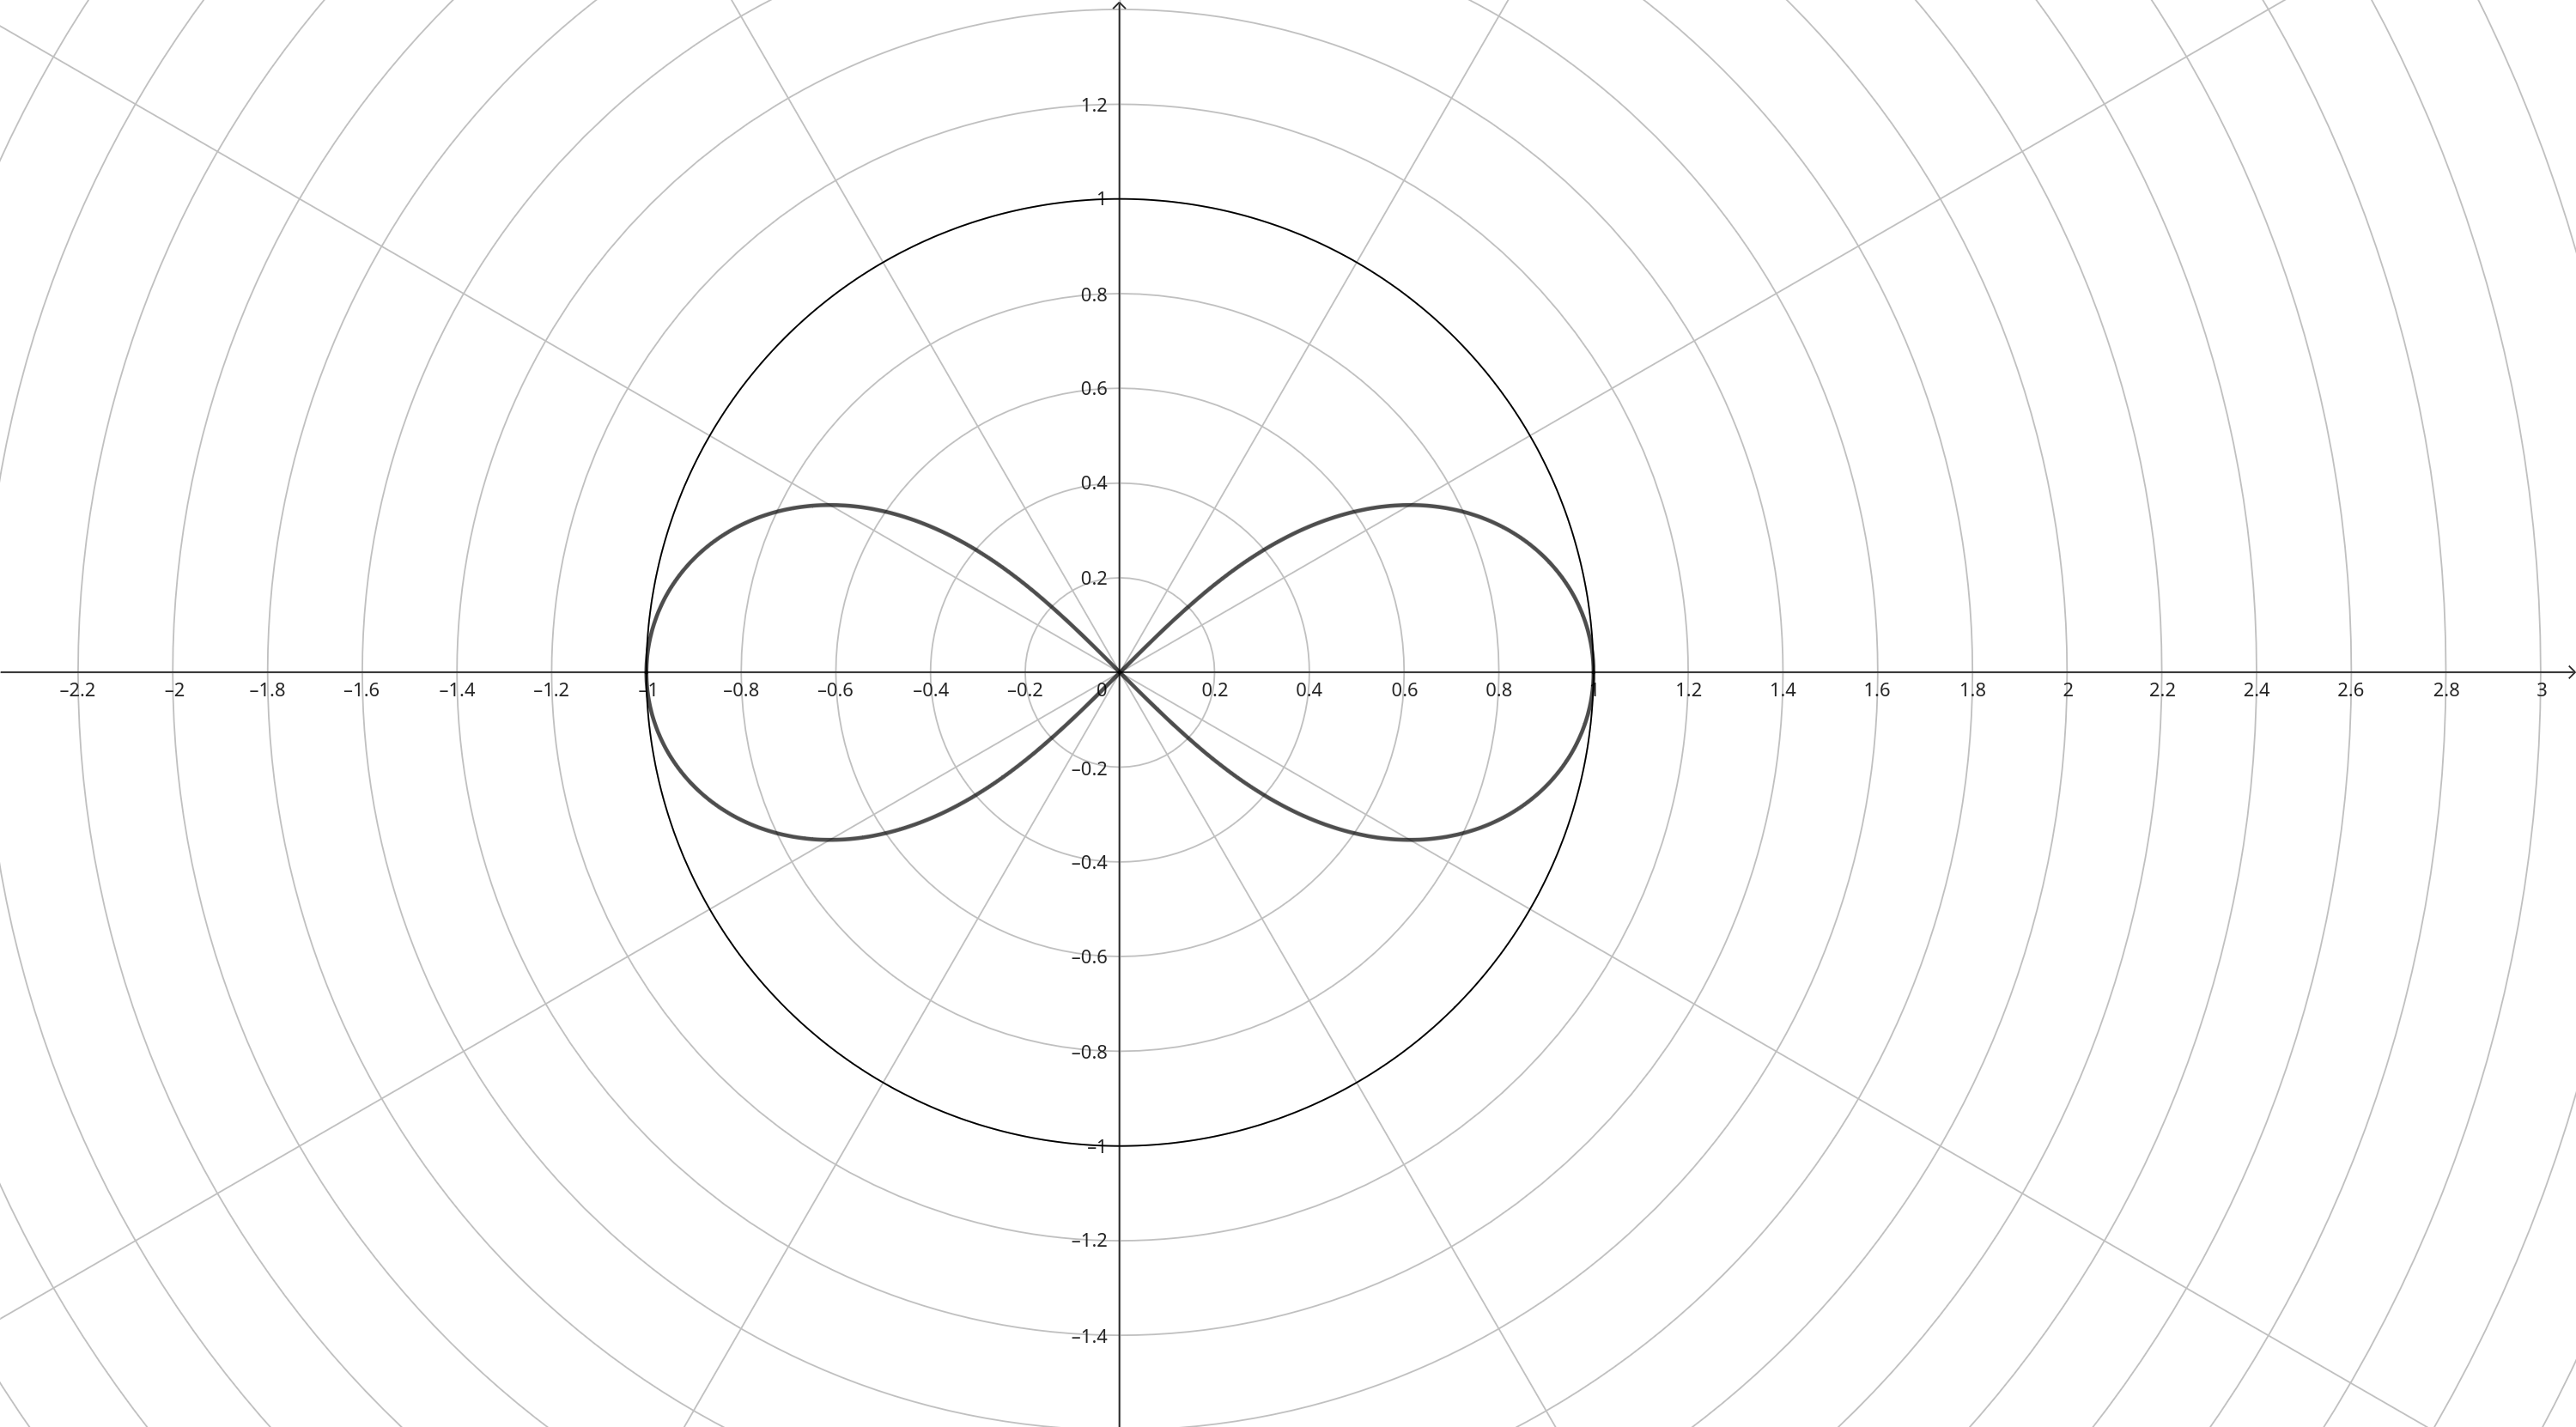
\includegraphics[width=\linewidth]{5F-2.5-rubin.cuypers.INF.png}\\
\end{figure}


\begin{thebibliography}{999}
%\bibitem{a} Referentie
\end{thebibliography}
\end{document} 
